\documentclass{beamer}

% Some common packages
\usepackage{graphicx, color}
\usepackage{alltt}
\usepackage{booktabs, calc, rotating}
\usepackage{natbib}
\usepackage{multicol}
\usepackage{amsmath, amsbsy, amssymb, amsthm, graphicx}
\usepackage[english]{babel}
\usepackage{xkeyval} 
\usepackage{xfrac}
\usepackage[normalem]{ulem}
\usepackage{fancyvrb} 
\usepackage{tikz, geometry, tkz-graph, xcolor}
\usepackage[latin1]{inputenc}
\usepackage{times}
\usepackage[T1]{fontenc}

% Some shortcuts
\newcommand{\cov}{\mathrm{cov}}
\newcommand{\dif}{\mathrm{d}}
\newcommand{\bigbrk}{\vspace*{2in}}
\newcommand{\smallbrk}{\vspace*{.1in}}
\newcommand{\midbrk}{\vspace*{1in}}
\newcommand{\red}[1]{{\color{red}#1}}
\newcommand{\blue}[1]{{\color{blue}#1}}
\newcommand{\green}[1]{{\color{green}#1}}
\newcommand{\calc}[1]{{\fbox{\mbox{#1}}}}
\newcommand{\Var}{\mathrm{Var}}%
\newcommand{\Cov}{\mathrm{Cov}}%

\usetheme[numbering=fraction, progressbar = frametitle]{metropolis}
% section page?
% \usetheme[sectionpage=none]{metropolis}
% place progressbar under frametitle?
% \usetheme[progressbar = frametitle]{metropolis}



% To center title?
\setbeamertemplate{title page}[default]
% To add a rectangle box for title?
% \setbeamercolor{titlelike}{parent = frametitle}   

% item color and shape
% \setbeamertemplate{itemize item}{\color{mDarkTeal}$\bullet$}
% \setbeamertemplate{itemize subitem}{\color{mDarkTeal}$\bullet$}
% \setbeamertemplate{itemize subsubitem}{\color{mDarkTeal}$\bullet$}

% UTD colors
\definecolor{warmgray10}{RGB}{118,106,98}
\definecolor{warmgray2}{RGB}{213,210,202}
\definecolor{warmgray1}{RGB}{230,230,230}
\definecolor{flameOrange}{RGB}{199,91,18}
\definecolor{ecoGreen}{RGB}{0,133,86}

% only change item color 
\setbeamercolor*{itemize item}{fg = mDarkTeal}
\setbeamercolor*{itemize subitem}{fg = mDarkTeal}
\setbeamercolor*{itemize subsubitem}{fg = mDarkTeal}
% enumerate color
\setbeamercolor*{enumerate item}{fg = mDarkTeal}
\setbeamercolor*{enumerate subitem}{fg = mDarkTeal}
\setbeamercolor*{enumerate subsubitem}{fg = mDarkTeal}
% description color
\setbeamercolor*{description item}{fg = mDarkTeal}
\setbeamercolor*{description subitem}{fg = mDarkTeal}
\setbeamercolor*{description subsubitem}{fg = mDarkTeal}

% define blocks
\newenvironment<>{problock}[1]{
  \begin{actionenv}#2
    \def\insertblocktitle{#1}
    \par
    \mode<presentation>{
      \setbeamercolor{block title}{fg = white, bg = ecoGreen} %mDarkTeal}
      \setbeamercolor{block body}{fg = black, bg = warmgray1}
    }
    \usebeamertemplate{block begin}}
  {\par\usebeamertemplate{block end}\end{actionenv}}

\newenvironment<>{defblock}[1]{
  \begin{actionenv}#2
    \def\insertblocktitle{#1}
    \par
    \mode<presentation>{
      \setbeamercolor{block title}{fg = white,bg = flameOrange} %mDarkBrown}
      \setbeamercolor{block body}{fg = black,bg = warmgray1}
    }
    \usebeamertemplate{block begin}}
  {\par\usebeamertemplate{block end}\end{actionenv}}

% \setbeamerfont{block title}{size={}}
% \setbeamercolor{titlelike}{parent=structure,bg=flameOrange!80!black,fg=white} % title
\mode
<all>

% fancy for Verbatim?
\fvset{frame = single, framesep = 1mm,fontfamily = courier,
  fontsize = \scriptsize, numbers = left, framerule = .3mm,
  numbersep = 1mm,commandchars = \\\{\}}

% reset text width
\setbeamersize{text margin left = 5pt,text margin right = 5pt}

\title[Short title]{Statistics for Biology and Health\\ Chapter 5 Topics in Univariate Estimation\\ 
}
\author[Author name]{Qi Guo}
% \institute[UTD]{Department of Mathematical Sciences \\ The University of Texas at Dallas}
\date{July 21,2019}
% UTD logo on title page
% \titlegraphic{\includegraphics[width=5cm]{mono_nsm_print_header.jpg}}
\titlegraphic{
\includegraphics[scale = .27]{UTDmono_NSM_header_RGB-1.png}}

\begin{document}

% default title thicker line
% need to adjust
% \frame{
% \maketitle
% \begin{tikzpicture}[remember picture, overlay]
%   \def\xmargin{.1cm}     % Left and right margin of the title line
%   \def\yshift{-0.1cm}   % Moves the title line upwards (-1.25cm moves title line downwards)
%   \draw[mLightBrown,line width=2pt] (current page.west) ++(\xmargin,\yshift) -- ++({\paperwidth-2*\xmargin},0);
% \end{tikzpicture}
% }

\frame{
  \vspace{1cm}
  \maketitle
  \begin{tikzpicture}[remember picture, overlay]
    \def\xmargin{.8cm}     % Left and right margin of the title line
    \def\yshift{0.6cm}   % Moves the title line upwards 
    \draw[mLightBrown,line width=2.2pt] (current page.west) ++(\xmargin,\yshift) -- ++({\paperwidth-2*\xmargin},0);
  \end{tikzpicture}
}


% Set up UTD backgroud
% Show background from here on
\setbeamercolor*{item}{fg=red}
\bgroup
\usebackgroundtemplate{
  \tikz[overlay,remember picture] \node[opacity=0.05, at=(current page.center)] {
    
\includegraphics[height=\paperheight,width=\paperwidth]{UTDbg}};}


\begin{frame}{Contents}
  \setbeamertemplate{section in toc}[sections numbered]
  \tableofcontents[hideallsubsections]
\end{frame}

\section{Introduction}
\begin{frame}{Introduction}
\begin{itemize}
\item Now we know KM estimator provides an estimate of the survival function, and NA estimator provides an estimate of the cumulative hazard rate, and the slope of the NA estimator provides a crude estimate of the hazard rate, but it usually hard to interpret.
\item But these two estimator provide limited information about the mechanism of the process under study, as summarized by the hazard rate, so use kernel-smoothing technique to provide a better estimator of the hazard rate, which based on the NA estimator $\tilde{H}(t)$ and its variance $\hat{V}[\tilde{H}(t)]$.  
\end{itemize}
\end{frame}
\begin{frame}{Introduction}
\begin{itemize}
\item Estimation techniques for both the additive and multiplicative models for excess mortality about the experience of the experimental subjects differs. 
\item In the end, show the problem of estimation of the survival function for right censored data is considered from a Bayesian perspective.
\end{itemize}
\end{frame}

\section{Estimating the Hazard Function}
\begin{frame}{Introduction}
\begin{itemize}
\item Now we know $\tilde{H}(t)$ is a step function with jumps at the event times, $0 = t_0 < t_1 < t_2 < \cdots < t_D$, let $\Delta \tilde{H}(t_i) = \tilde{H}(t_i) - \tilde{H}(t_{i-1})$ and $\Delta \hat{V}(\tilde{H}(t_i)) =\hat{V}(\tilde{H}(t_i) - \hat{V}(\tilde{H}(t_{i-1})$ 
\item Note that $\Delta \hat{V}(\tilde{H}(t_i))$ provides a crude estimator of $h(t)$ at the death times. The kernel-smoothed estimator of $h(t)$ is a weighted average of these crude estimates over event times close to $t$.
\item Closeness is determined by a bandwidth $b$, so that event times in the range $t-b$ to $t+b$ are included in the weighted average which estimates $h(t)$.
\item The bandwidth is chosen either to minimize some measure of the mean-squared error or to give a desired degree of smoothness
\end{itemize}
\end{frame}

\begin{frame}{The kernel function}
\begin{itemize}
\item The weights are controlled by the choice of a kernel function, $K( )$,defined on the interval $[-1, +1]$, which determines how much weight is given to points at a distance from $t$.
\item Common choices for the kernel are the uniform kernel with
\begin{equation*}
K(x) = 1/2 \  \ for \  -1\le x \le +1
\end{equation*}
\item The Epanechnikov kernel with
\begin{equation*}
K(x) = 0.75(1-x^2) \ \ for  \ -1\le x \le +1
\end{equation*}
\item The biweight kernel with
\begin{equation*}
K(x) = 0.75(1-x^2) \ \ for  \ -1\le x \le +1
\end{equation*}
\item The uniform kernel gives equal weight to all deaths in the interval $t-b$ to $t+b$, whereas the other two kernels give progressively heavier weight to points close to $t$.
\end{itemize}
\end{frame}

\begin{frame}{The kernel-smoothed hazard rate estimator}
\begin{itemize}
\item For any $t>0$, for which $b \le t \le t_D -b$, the kernel smoothed estimator of $h(t)$ based on the kernel $K()$ is given by: 
\begin{equation*}
\hat{h}(t) = b^{-1} \sum_{i=1}^{D} K(\frac{t-t_i}{b}) \Delta \tilde{H}(t_i)
\end{equation*}
\item The variance of $\hat{h}(t)$ is estimated by:
\begin{equation*}
\delta ^2 [\hat{h}(t)] = b^{-2} \sum_{i=1}^{D} {K(\frac{t-t_i}{b})}^2 \Delta \hat{V}(\tilde{H}(t_i))
\end{equation*}
\item When $t<b$, there are no events times less than 0 are observable, the use of an asymmetric kernel is suggested.
\end{itemize}
\end{frame}

\begin{frame}{Gasser and Muller modified kernels}
\begin{itemize}
\item Let $q = t/b$, define a modified kernel which accounts for the restricted range of the data, for the uniform kernel are expressed by:
\begin{equation*}
K_q(x) = \frac{4(1+q^3)}{(1+q^4)} + \frac{6(1-q)}{(1+q)^3} x \ \ \ for\ -1 \le x \le q
\end{equation*}
\item And we also have versions for the Epanechnikov kernel and the biweight kernel.
\item The confidence intervals or confidence bands for the hazard rate based on the smoothed hazard rate estimate is :
\begin{equation*}
\hat{h}(t)exp\bigg[\pm \frac{Z_{1-\alpha/2} \sigma(\hat{h}(t))}{\hat{h}(t)} \bigg]
\end{equation*}
for a $(1-\alpha) \times 100\%$ pointwise CI based on a log transformation.
\end{itemize}
\end{frame}

\begin{frame}{Example}
\begin{itemize}
\item \texttt{Figure 6.3} shows the estimated hazard rate based on a bandwidth of 1 year for the uniform, Epanechnikov, and biweight kernels.  
\begin{figure}
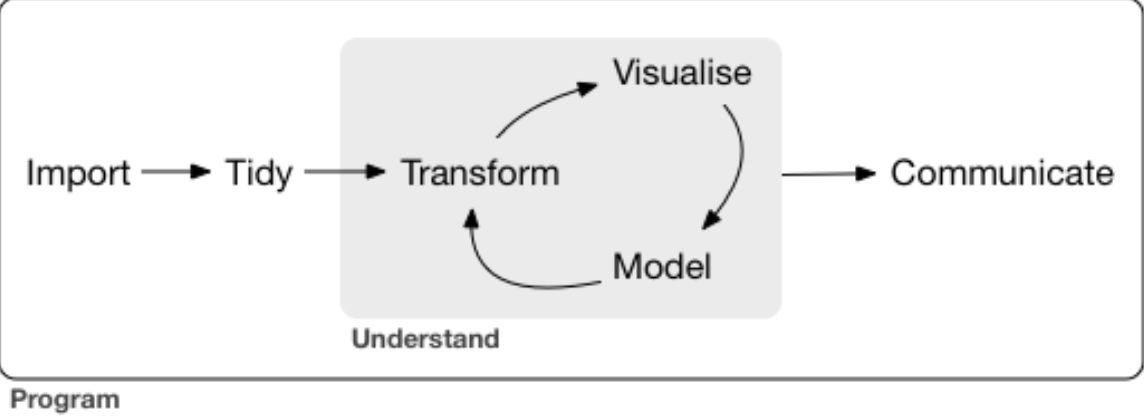
\includegraphics[scale = .3]{001.png}
\end{figure}
\end{itemize}
\end{frame}

\begin{frame}{Determine the bandwidth}
\begin{itemize}
\item Using kernel smoothing to obtain an estimate of the hazard rate is selection of the proper bandwidth.
\item One way to pick a good bandwidth is to use a cross-validation technique for determining the bandwidth that minimizes some measure of how well the estimator performs. 
\item One such measure is the mean integrated squared error $(MISE)$ of $\hat{h}$ over the range $\tau_L$ to $\tau_U$ defined by:
\begin{equation*}
\begin{split}
MISE(b) &= E \int_{\tau_L}^{\tau_U} [\hat{h}(u) - h(u)]^2 du \\ &= E [ \int_{\tau_L}^{\tau_U} \hat{h}^2(u)du] - 2 E[\int_{\tau_L}^{\tau_U} \hat{h}(u)h(u)du] + E [ \int_{\tau_L}^{\tau_U} h^2(u)du] 
\end{split}
\end{equation*}
\end{itemize}
\end{frame}

\begin{frame}{Determine the bandwidth}
\begin{itemize}
\item The first term can be estimated by $\int_{\tau_L}^{\tau_U} \hat{h}^2(u)du$. If we evaluate $
\hat{h}$ at a grid of points $\tau_L = u_1 < \cdots <u_M = \tau_U$, then, an approximation to this integral by the trapezoid rule is $\sum_{i=1}^{M-1}(\frac{u_{i+1} - u_i}{2})[\hat{h}^2(u_i)+\hat{h}^2(u_{i+1})]$.
\item The second term can be estimated by a cross-validation estimate suggested by Ramlau-Hansen. This estimate is  $b^{-1}\sum_{i \neq j}^{}K(\frac{t_i - t_j}{b})\Delta \tilde{H}(t_i)\Delta \tilde{H}(t_j)$, where the sum is over the event times between $\tau_L$ and $\tau_U$.
\item The last term depends on the unknown
hazard rate, it is independent of the choice of the kernel and the bandwidth and can be ignored when finding the best value of $b$.
\end{itemize}
\end{frame}


\begin{frame}{Determine the bandwidth}
\begin{itemize}
\item Thus to find the best value of $b$ which minimizes the $MISE$ for a fixed kernel, find $b$ which minimizes the function:
\begin{equation*}
\begin{split}
g(b) &= \sum_{i=1}^{M-1} \bigg( \frac{u_{i+1} - u_i}{2}\bigg) [ \hat{h}^2(u_i) + \hat{h}^2(u_{i+1})] \\ &-2 b^{-1} \sum_{i\neq j}^{}K \bigg( \frac{t_i - t_j}{b}\bigg) \Delta \tilde{H}(t_i) \Delta \tilde{H}(t_j)
\end{split}
\end{equation*}
\end{itemize}
\end{frame}

\begin{frame}{Example}
\begin{itemize}
\item \texttt{Figure 6.4} shows the effects of changing the bandwidth on the estimate of $h(t)$. In this figure, based on the Epanechnikov kernel, we see that increasing the bandwidth provides smoother estimates of the hazard rate. 
\begin{figure}
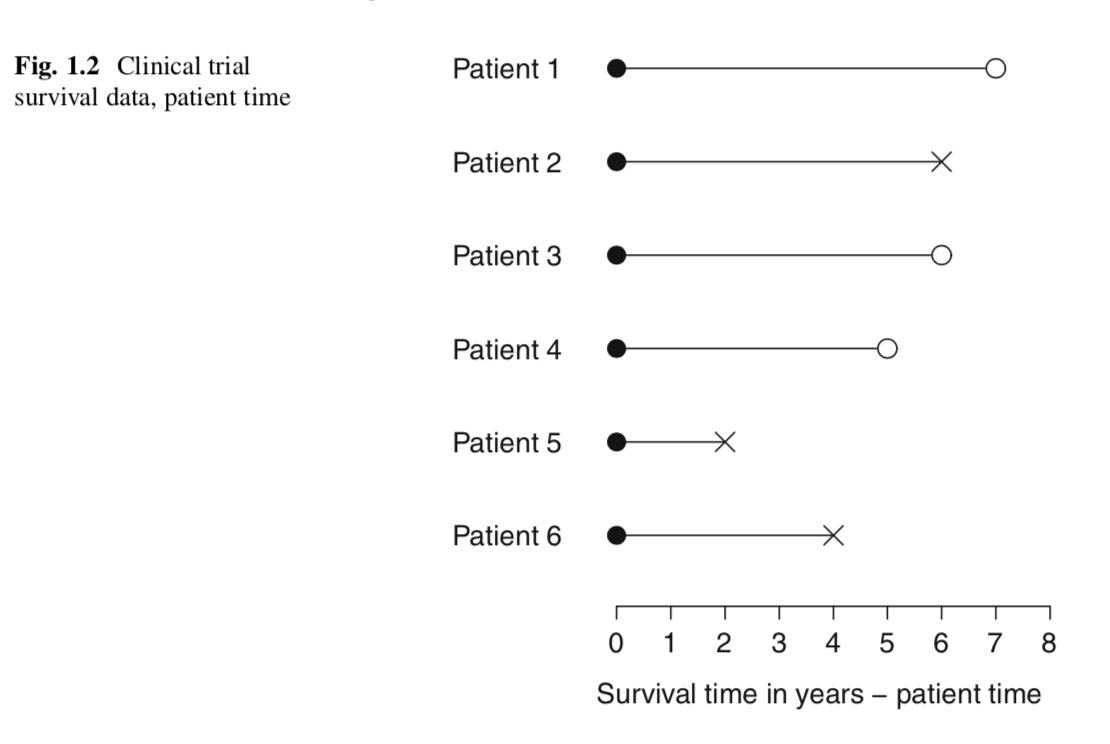
\includegraphics[scale = .28]{002.png}
\end{figure}
\end{itemize}
\end{frame}

\section{Estimation of Excess Mortality}
\begin{frame}{Introduction}
\begin{itemize}
\item Sometimes it's of interest to compare the mortality experience of a group of individuals to a known standard survival curve.
\item Two simple models have been proposed to provide an inference on how the study population's mortality differs from that in the reference population.
\item Suppose we have data on $n$ individuals. Let $\theta_j(t)$ be the reference hazard rate for the $j$th individual in the study, which typically depends on the characteristics of the $j$th patient, such as race,sex,age,etc.
\end{itemize}
\end{frame}

\begin{frame}{The relative mortality model}
\begin{itemize}
\item The first model for excess mortality, commonly known as the relative mortality model, assumes that the hazard rate at time $t$ for the $j$th patient under study conditions, $h_j(t)$, is a multiple,$\beta(t)$, of the reference hazard rate for this individual:
\begin{equation*}
h_j(t) = \beta(t)\theta_j(t) \ \ j = 1,2,\cdots, n
\end{equation*}
\item If $\beta(t) > 1$, individuals in the study group are experiencing the event of interest at a faster rate than comparable individuals in the reference population
\item Let $B(t) = \int_{0}^{t}\beta(u)du$ be the cumulative relative excess mortality.
\item The data available for estimating $B(t)$, for each individual, consists of study times and death indicators.
\end{itemize}
\end{frame}

\begin{frame}{The relative mortality model}
\begin{itemize}
\item For the $j$th individual, let $Y_j(t)$ be 1 if the individual is at risk at time $t$ and 0, otherwise.Define the function $Q(t)= \sum_{j=1}^{n}\theta_j(t)Y_j(t)$, let $t_1 < t_2 < \cdots < t_D$ be the times at which the events occur  and $d_i$ the number of events observed at time $t_i$. The estimator of $B(t)$ and its variance are:
\begin{equation*}
\hat{B}(t) = \sum_{t_i \le t}^{}\frac{d_i}{Q(t_i)}
\end{equation*}	
and
\begin{equation*}
\hat{V}[\hat{B}(t)] = \sum_{t_i \le t}^{}\frac{d_i}{{Q(t_i)}^2}
\end{equation*}	
\item And we can also find the CI or CB, and a crude estimator of the relative risk function $\beta(t)$ is given by the slope of the estimated cumulative risk mortality estimator, and it can also improved by kernel smoothing like before.
\end{itemize}
\end{frame}



\begin{frame}{The additive mortality model}
\begin{itemize}
\item A second model used for comparing the study population to a reference population is the excess or additive mortality model.
\item Assume that the hazard rate at time $t$ for the $j$th individual under study is a sum of the population mortality rate $\theta_j(t)$ and an excess mortality function $\alpha(t)$.
\item The $\alpha(t)$ is same for all individuals in the study group, and it's positive means study patients are dying faster than those in the reference population, is expressed by:
\begin{equation*}
h_j(t) = \alpha(t) +\theta_j(t) \ \ j =1, \cdots, n
\end{equation*}
\item Introduce the cumulative excess mortality function for convenient to estimate the $\alpha()$:
\begin{equation*}
A(t) = \int_{0}^{t} \alpha(u)du
\end{equation*}
\end{itemize}
\end{frame}


\begin{frame}{The additive mortality model}
\begin{itemize}
\item The estimator of $A(t)$ is constructed from the difference of the observed hazard rate, estimated by the ordinary NA estimator $\tilde{H}(t)$ and  an ``expected'' cumulative hazard rate $\Theta(t)$ based on the reference hazard rates.
\begin{equation*}
\Theta(t) = \sum_{j=1}^{n} \int_{0}^{t} \theta_j(u)\frac{Y_j(u)}{Y(u)}du
\end{equation*}
where $Y(t) = \sum_{j=1}^{n}Y_j(t)$ is the number of at risk at time $t$.
\item The estimated variance is 
\begin{equation*}
\hat{V}[\hat{A}(t)] = \sum_{t_i \le t}^{}\frac{d_i}{{Y(t)}^2}
\end{equation*}
\item  The survival cure, $S^*(t) = \exp[-\Theta(t)]$, provides an estimate of the expected survival curve if the reference mortality model is the same as the study population.
\end{itemize}
\end{frame}

\section{Bayesian Nonparametric Methods}
\begin{frame}{Introduction}
\begin{itemize}
\item An alternative to the classical nonparametric approach to estimating the survival function is to use Bayesian nonparametric methods.
\item An investigator's a priori belief in the shape of the survival function is combined with the data to provide an estimated survival function.
\item The parameters of the model are treated as random variables selected from the prior distribution,which is a multivariate distribution on the parameters, is selected to reflect the investigator's prior belief in the values of the parameters. 
\item It's complicated and just introduce the crude steps of the Bayesian methods, more details in P187-P197.
\end{itemize}
\end{frame}

\begin{frame}{Two classes of prior distributions}
\begin{itemize}
\item To obtain an estimate of the survival function, specify a loss function on which to base the decision rule.Analogous to the simple parametric case, use the squared-error loss function:
\begin{equation*}
L(S,\hat{S}) = \int_{0}^{\infty} [\hat{S}(t)-S(t)]^2 d \omega(t)
\end{equation*}
where $\omega(t)$ is a weight function.
\item For this loss function, the value of $\hat{S}$, which minimizes the posterior expected value of $L(S,\hat{S})$, is the posterior mean and the Bayes risk $E[L(S, \hat{S})|DATA]$ is the posterior variance.
\item And we have two classes of prior distributions.
\end{itemize}
\end{frame}

\begin{frame}{Two classes of prior distributions}
\begin{itemize}
\item Both lead to closed form estimates of the survival function using the squared-error loss function.
\item These priors are chosen because they are conjugate priors for either the survival function or the cumulative hazard function. For a conjugate prior, the prior and posterior distributions are in the same family.
\item The first prior is for the survival function, for this prior, we assume that the survival function is sampled from a Dirichlet process with a parameter function $\alpha$.
\item A second prior is to provide a prior distribution for the cumulative hazard function $H(t) = - \ln[S(t)]$. Here, we shall use a beta process prior. 
\end{itemize}
\end{frame}

\begin{frame}{Monte Carlo Bayesian methods}
\begin{itemize}
\item The Monte Carlo Bayesian methods or the Gibbs sampler is more flexible than the other two approaches.
\item For right-censored data,the closed form estimates of the survival function are available. But for other censoring or truncation schemes, such simple estimates are not available.
\item The Monte Carlo Bayesian methods provides a way of simulating the desired posterior distribution of the survival function.
\end{itemize}
\end{frame}

\end{document}